\documentclass[]{final_report}
\usepackage{graphicx}
\usepackage{hyperref}
\usepackage{titlesec}
\usepackage[utf8]{inputenc}
\usepackage[backend=biber, style=ieee]{biblatex}
\usepackage{amsmath}
\usepackage{amssymb}
\usepackage{float}
\usepackage{tabularx} % Needed for the X column type
\usepackage{booktabs} % For prettier tables
\usepackage{lipsum}   % For dummy text
\usepackage{xcolor}  % for custom colors
\usepackage{adjustbox}
\usepackage{tikz}
\usepackage{rotating}
\usepackage{pdflscape}
\usepackage{fancyhdr}
\usepackage{longtable}
\fancypagestyle{lscape}{%
  \fancyhf{} % clear all header and footer fields
  \fancyfoot[LE,RO]{\makebox[0pt][l]{\rotatebox[origin=c]{90}{\thepage}}} % Left Even, Right Odd
  \renewcommand{\headrulewidth}{0pt}
  \renewcommand{\footrulewidth}{0pt}
}



\addbibresource{fyp.bib}
\usepackage{amsthm}
\theoremstyle{definition}
\newtheorem{definition}{Definition}[chapter]
\newtheorem{basic}{Basic Definition}

%%%%%%%%%%%%%%%%%%%%%%
%%% Input project details
\def\studentname{Jude Asare}
\def\reportyear{2023/2024}
\def\projecttitle{Implementing the PKCS\#1 v1.5 Signature Scheme with provably secure parameters}
\def\supervisorname{Saqib Kakvi}
\def\degree{MSci (Hons) in Computer Science (Information Security)}
\def\fullOrHalfUnit{Appendix A} 
\begin{document}


%%%%%%%%%%%%%%%%%%%%%%
%%% Table of Contents
\tableofcontents\pdfbookmark[0]{Table of Contents}{toc}\newpage





\chapter{Appendix A Software Development of Proof of Concept program}



\section{Appendix A.2 Requirements and Analysis}
The overall goal of the system is to provide primarily, a basic implementation of the PKCS signature scheme from which a user can interact with via a user interface to perform relevant actions. The program will also include the other considered schemes, to be integrated once the implementation for the PKCS scheme has been established.
The core actions comprise, the generation of keys, creation of signatures and finally verification of previously created signatures. 
The program will form the foundation for the eventual delivery of the benchmarking program used to examine the discussed provable security overhead.

\subsection{Description of Actors}
\begin{table}[H]
    \centering
    \caption{Description of Actors for the POC Digital Signature Program}
    \label{tab:actors_description}
    \begin{tabular}{|l|p{10cm}|}
    \hline
    \textbf{Actor / Role Name} & \textbf{Role Description and Objective} \\
    \hline
    User/Signer & Individual who wishes to digitally sign a piece of content. The signer generates key pairs, can input content, and create a digital signature using their private key. Their main goal is to ensure that the content they're signing is authenticated and its integrity is maintained, proving that it hasn't been tampered with. \\
    \hline
    Verifier & Entity that needs to validate the authenticity and integrity of a digitally signed piece of content. The verifier inputs signed content, a corresponding public key, and attempts to verify a specified digital signature. Their primary objective is to ascertain that the content hasn't been altered post-signing and to confirm the identity of the signer. \\
    \hline
    \end{tabular}
\end{table}


\subsection{User Stories}
\textbf{Essential Requirements}
\begin{enumerate}
\item Potential signer should be able to generate and retrieve a public-private key pair having provided a key size.
\begin{itemize}
\item User should be presented with a text box to input the key size.
\item The system should handle any exceptions or errors during key generation, displaying to the user of any issues.
\item The system should notify the signer once the key generation process is successful.
\item Once the key is generated the user should have the option to save it to a file.
\end{itemize}
\item Having provided a message and private key, the signer should be able to retrieve the resulting computed digital signature.
\begin{itemize}
\item The signer should be presented with a text box to input the message intended for signing.
\item The signer should be able to specify and input the private key using file selection via a browse option.
\item The system should handle any exceptions or errors during signature generation, displaying to the signer of any issues.
\item The system should notify the signer once the signing process is successful.
\item Once the signature is generated the signer should have the option to copy the signature to the clipboard or save it to a file.
\end{itemize}
\item Having provided a message, its corresponding digital signature, and a public key, the verifier should be able to verify the authenticity of the signature.
\begin{itemize}
\item The verifier should be presented with a text box or file browse option to input the message corresponding to the signature intended for verifying.
\item The verifier should be presented with a file browse option to input the signature intended for verifying.
\item The system should handle any exceptions or errors during verification process, displaying to the verifier of any issues.
\item The system should notify the verifier once the verification process is successful.
\end{itemize}
\item The signer should be able to sign messages using the PKCS\#1 v1.5 Signature Scheme.
\item The verifier should be able to verify messages using the PKCS\#1 v1.5 Signature Scheme.
\item The signer should be able to sign messages using the ANSI X9.31 rDSA Signature Scheme.
\item The verifier should be able to verify messages using the ANSI X9.31 rDSA Signature Scheme.
\item The signer should be able to sign messages with partial or full recovery using the ISO/IEC 9796-2:2010 Signature Scheme 1.
\item The verifier should be able to verify messages with partial or full recovery using the ISO/IEC 9796-2:2010 Signature Scheme 1.
\end{enumerate}

\textbf{Non Essential Requirements}
\begin{enumerate}
\item[] Performance
\begin{enumerate}
\item[7.] User shoulder be able view a measurement of time taken for each of the signature related operations i.e., Key generation, Signature creation and verification.
\item[] Non Functional
\begin{itemize}
\item[8.] The program should generate keys within a reasonable timeframe.
\item[9.] The program should create signatures within a reasonable timeframe.
\item[10.] The program should verify signatures within a reasonable timeframe.
\end{itemize}
\end{enumerate}
\end{enumerate}

\subsection{UML Use Case}
\begin{figure}[H]
    \centering
    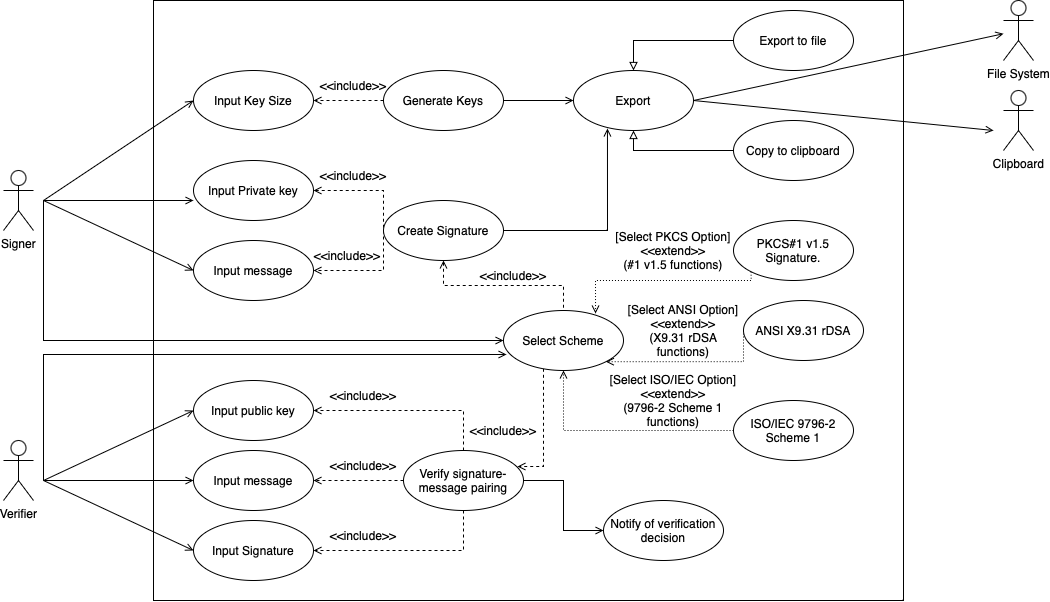
\includegraphics[scale=0.48]{POC_USE-CASE.png}
    \caption{UML Use Case Diagram}
    \label{fig:uc}
\end{figure}



\textbf{Generate Keys Use Case}

\noindent\textbf{Flow of Events:}
\begin{enumerate}
    \item User selects "Generate Key" from the main menu options panel.
    \item User is presented with an input box labeled "Input Key Size".
    \item User inputs desired key size into the box.
    \item System processes the request and generates the public-private key pair.
    \item System displays a notification informing the user that the key generation process was successful.
    \item User is presented with options "Export to file" and "Copy to clipboard" for the signature.
    \item User selects desired option to either save the keys to a file or copy them to clipboard.
\end{enumerate}

\noindent\textbf{Alternative flows:}
\begin{enumerate}
    \item[3a.] User inputs an invalid key size.
    \begin{enumerate}
        \item[3a1.] System warns user about the invalid input and prompts them to enter a valid key size again.
    \end{enumerate}
    \item[5a.] System encounters an error during key generation.
    \begin{enumerate}
        \item[5a1.] System displays an error message and prompts the user to try again.
    \end{enumerate}
     
\end{enumerate}



\textbf{Create Signature Use Case}

\noindent\textbf{Flow of Events:}
\begin{enumerate}
    \item User selects "Sign message" from the main menu options panel.
    \item User is presented with text boxes labeled "Input Private Key" and "Input Message".
    \item User inputs their private key and the message they wish to sign.
    \item User selects the desired signature scheme from options like "PKCS\#1 v1.5 Signature", "ANSI X9.31 rDSA", etc.
    \item System processes the input and computes the digital signature.
    \item System displays a notification informing the signer that the signing process was successful.
    \item User is presented with options "Export to file" and "Copy to clipboard".
    \item User selects desired option to either save the keys to a file or copy them to clipboard.
\end{enumerate}

\noindent\textbf{Alternative flows:}
\begin{enumerate}
    \item[3a.] User inputs an invalid or mismatched private key.
    \begin{enumerate}
        \item[3a1.] System warns user about the invalid input and prompts them to enter a valid key.
    \end{enumerate}
    \item[5a.] System encounters an error during signature creation.
    \begin{enumerate}
        \item[5a1.] System displays an error message and prompts the user to try again.
    \end{enumerate}
    \item[7a.]  User selected an ISO\slash IEC 9796-2 scheme in step 4.
    \begin{enumerate}
        \item[7a1.] User is presented with options "Export to file" and "Copy to clipboard" for the computed signature and additionally if applicable. a computed non recoverable portion of their initially submitted message.
    \end{enumerate}
\end{enumerate}

\textbf{Verify Signature Use Case}

\noindent\textbf{Flow of Events:}
\begin{enumerate}
    \item User selects "Verify Signature" from the main menu options panel.
    \item User selects the desired signature scheme from options like "PKCS\#1 v1.5 Signature", "ANSI X9.31 rDSA", etc..
    \item User is presented with options to input the message, its corresponding signature, and the public key
    \item User provides all required inputs.
    \item System processes the information and verifies the authenticity of the signature.
    \item System displays a notification with the result, either confirming the authenticity or notifying of a mismatch.
\end{enumerate}

\noindent\textbf{Alternative flows:}
\begin{enumerate}
 \item[3a.]  User selected the ISO\slash IEC 9796-2 scheme 1 with full message recovery option scheme in step 2.
    \begin{enumerate}
        \item[3a1.] System greys out box requiring message input so that user cannot input a message.
    \end{enumerate}
  \item[3b.]  User selected the ISO\slash IEC 9796-2 scheme 1 with partial message recovery option scheme in step 2.
    \begin{enumerate}
        \item[3b1.] System changes the displayed label for message input to non-recoverable message portion.
    \end{enumerate}
    \item[4a.] User inputs mismatched or incorrect information.
    \begin{enumerate}
        \item[4a1.] System warns user about the incorrect input and suggests rechecking the inputs.
    \end{enumerate}
    \item[5a.] System encounters an error during verification.
    \begin{enumerate}
        \item[5a1.] System displays an error message and prompts the user to try again.
    \end{enumerate}
    \item[6a.]  User selected an ISO\slash IEC 9796-2 scheme in step 2.
    \begin{enumerate}
        \item[6a1.] User is presented with options "Export to file" and "Copy to clipboard" for the computed signature and additionally if applicable a recovered portion of a message submitted some time in the past to the signature generation process.
    \end{enumerate}
\end{enumerate}

\subsection{Acceptance Tests}

\textbf{1. Key Pair Generation:}
\begin{enumerate}
\item Open the application and locate the key generation section.
\item Input a valid key size into the provided text box and submit.
\item If key size is invalid no key is issued and the user is informed to try again. 
\item Observe that no exceptions or errors are displayed during the key generation process.
\item If there are errors during key generation the user is informed to try again.
\item Confirm that a notification is presented to the user upon successful key generation.
\item Check if there is an option to save the generated key pair to a file and perform a successful save.
\end{enumerate}

\textbf{2. Digital Signature Generation:}
\begin{enumerate}
\item Locate the signature generation section in the application.
\item Input a test message into the provided text box.
\item Use the browse option to provide a valid private key file.
\item If empty message or invalid file is provided, the user is informed to try again. 
\item Ensure no errors or exceptions are displayed during the signing process.
\item Confirm that a notification is presented to the signer upon successful signature generation.
\item Check for options to either copy the signature to clipboard or save it to a file and verify both functionalities.
\end{enumerate}

\textbf{3. Digital Signature Verification:}
\begin{enumerate}
\item Locate the signature verification section in the application.
\item Use the text box or file browse option to input the original test message.
\item Use the browse option to provide the generated signature file.
\item If empty message or invalid file is provided, the user is informed to try again. 
\item Ensure no errors or exceptions are displayed during the verification process.
\item Confirm that a notification is presented to the verifier upon successful verification.
\end{enumerate}

\textbf{4. Signature and Verification with PKCS\#1 v1.5:}
\begin{enumerate}
\item Set the application to use the PKCS\#1 v1.5 Signature Scheme.
\item Sign a test message and verify its signature using the previous steps. Ensure both processes succeed.
\end{enumerate}

\textbf{5. Signature and Verification with ANSI X9.31 rDSA:}
\begin{enumerate}
\item Set the application to use the ANSI X9.31 rDSA Signature Scheme.
\item Sign a test message and verify its signature using the previous steps. Ensure both processes succeed.
\end{enumerate}

\textbf{6. Signature Generation with ISO/IEC 9796-2:2010 Scheme 1:}
\begin{enumerate}
\item Set the application to use the ISO/IEC 9796-2:2010 Signature Scheme 1.
\item Locate the signature generation section in the application.
\item Input a test message into the provided text box. 
\item Use the browse option to provide a valid private key file.
\item If empty message or invalid file is provided, the user is informed to try again. 
\item Ensure no errors or exceptions are displayed during the signing process.
\item Confirm that a notification is presented to the signer upon successful signature generation.
\item Check and verify separate options (copying to clipboard and saving to a file) for the signature.
\item Check and verify separate options (copying to clipboard and saving to a file) for non message portion if if user submitted a sufficiently short message relative to modulus (if message is too short there is no non recoverable portion).
\end{enumerate}

\textbf{6. Signature Verification with ISO/IEC 9796-2:2010 Scheme 1}
\begin{enumerate}
\item Set the application to use a variant of ISO/IEC 9796-2:2010 Signature Scheme 1.
\item Locate the signature verification section in the application.
\item Use the browse option to provide the generated signature file.
\item Use the text box or file browse option to input the original test message if user did received a non recoverable message from previous signature generation process
\item Ensure no errors or exceptions are displayed during the verification process.
\item Confirm that a notification is presented to the verifier upon successful verification.
\item Check and verify separate options (copying to clipboard and saving to a file) for  recoverable message portion if user submitted a legitimate non recoverable message portion to the verification process in step 4.
\end{enumerate}

\section{Appendix A.3 Design}
\subsection{Program packages}
\begin{figure}[H]
    \centering
    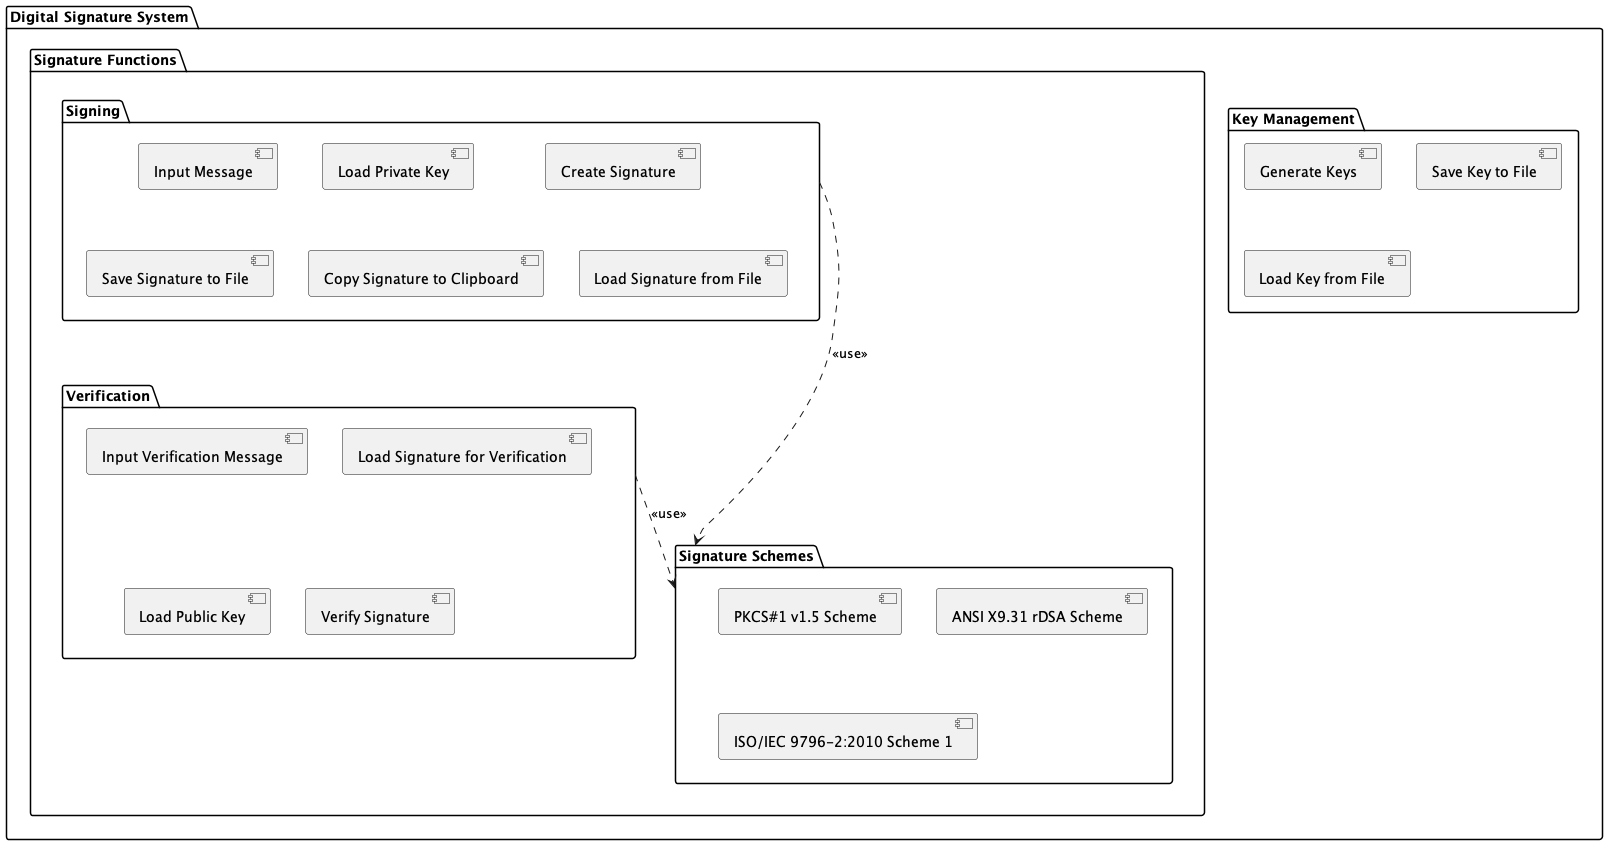
\includegraphics[scale=0.31]{package.png}
    \caption{POC program Packages}
    \label{fig:pack}
\end{figure}
Figure \ref{fig:pack} depicts the core functionality of the POC program and is in direct alignment with previously elaborated on (see requirements) user activities of signing, creating keys, and verifying, using a specified scheme like PKCS\#1-v1.5.
\subsection{UML sequence diagram}
\begin{figure}[H]
    \centering
    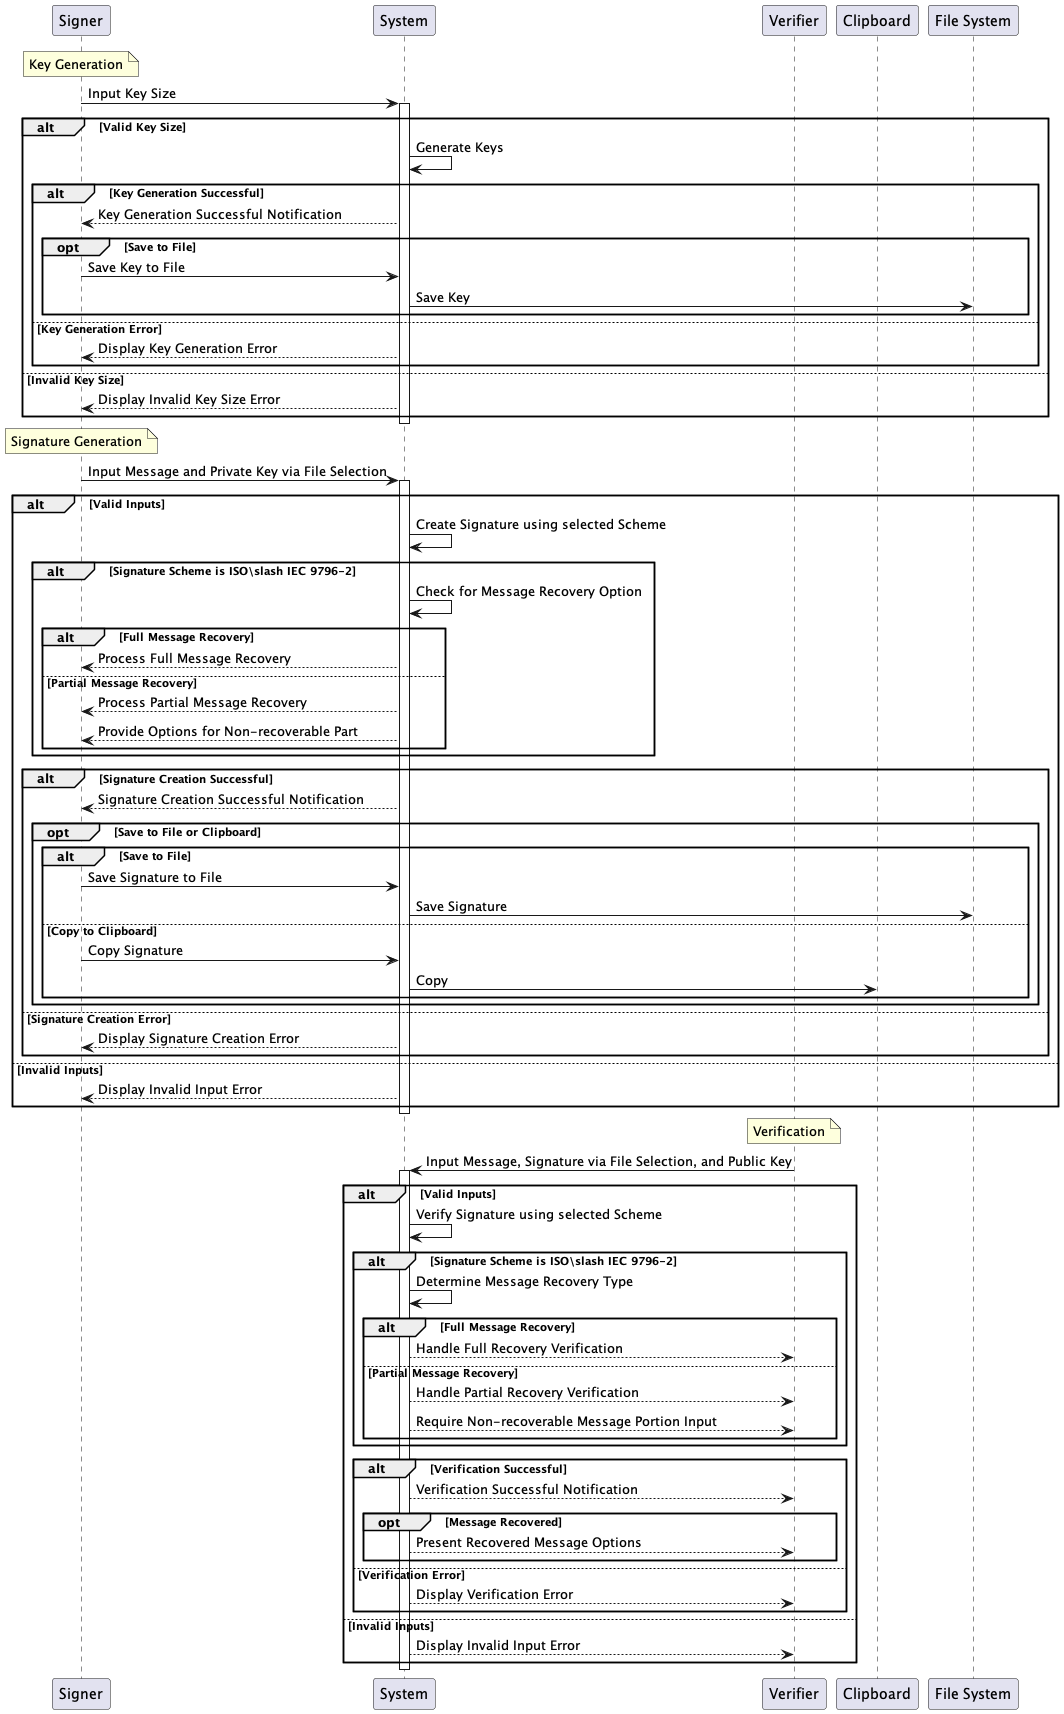
\includegraphics[scale=0.38]{seq2.png}
    \caption{UML Sequence Diagram}
    \label{fig:uc}
\end{figure}
The above diagram is mostly a high level view of the core behaviour that can be expected to performed by a user of the proof of concept of program. The point at which the diagram departs this is the specialised functionality to related to the message recovery signature schemes of the ISO standard. These schemes require special consideration because the related behaviour differs from the standard digital signature process. The ISO/IEC 9796-2 schemes incorporate message recovery features, where part or all of the original message can be reconstructed from the signature itself. This necessitates additional logic in both the signing and verifying processes. For partial message recovery, the signer needs to manage the non-recoverable portion of the message, ensuring that it is correctly returned alongside the signature. Subsequently they may then input the non-recoverable portion as part of their interaction with the verification process in attempt to recover the remaining portion of message. For full message recovery, the entire message is embedded in the signature, eliminating the need for a separate message input during verification but requiring careful handling to extract and validate the message from the signature. These nuances demand specialised user interfaces and system checks, making the ISO schemes distinct in their interaction and processing requirements within the application.

Initially, the user is prompted to generate cryptographic keys, providing a key size that, if valid, leads to the creation of a private and public key pair. The user can then opt to save these keys onto their file system.
Once keys are in place, the user can sign a message. They input the message into the system and load their private key. If the inputs are correct, the system employs a chosen signature algorithm to create a digital signature, which the user can save or copy to their clipboard. In case of invalid input or an error during signature creation, the user is informed with an error message.

For verification, the user inputs a message, loads the digital signature and the corresponding public key. The system checks the signature against the message using the public key. If the signature is valid, a success notification is displayed; otherwise, the user is alerted to a verification error. Throughout this process, the system guides the user with notifications or error messages based on the success or failure of the operations performed.
\section{System Testing}
\begin{table}[H]
  \caption{Test Cases}
  \centering

  \label{tab:table1}
  \resizebox{\textwidth}{!}{%
    \begin{tabular}{|l|p{2.5cm}|p{2.5cm}|p{2.5cm}|p{2.5cm}|p{3.5cm}|}
      \hline
      \textbf{Test ID} & \textbf{Prerequisites} & \textbf{Test Steps} & \textbf{Test Data} & \textbf{Expected Result} & \textbf{Actual Result}\\
      \hline
      MainMenu-001 & Application is launched and the user is presented with the main menu. & Click on the "[K] Generate Keys" button. & N/A & The application should navigate to the key generation page without errors. & \\
      \hline
      MainMenu-002 & Application is launched and the user is presented with the main menu. & Click on the "[S] Sign Document" button. & N/A & The application should navigate to the signature creation page without errors. & \\
      \hline
      MainMenu-003 & Application is launched and the user is presented with the main menu. & Click on the "[V] Verify Signature" button. & N/A & The application should navigate to the signature verification page without errors. & \\
      \hline
    \end{tabular}%
  }
\end{table}


\begin{longtable}{|l|p{2.5cm}|p{2.5cm}|p{2.5cm}|p{2.5cm}|p{3cm}|}
  \hline
  \textbf{Test ID} & \textbf{Prerequisites} & \textbf{Test Steps} & \textbf{Test Data} & \textbf{Expected Result} & \textbf{Actual Result} \\
  \hline
  KeyGen-001 & Application is installed and operational; the user is on the Key Generation page. & Navigate to the "Generate Keys" section. Enter a valid bit size in the input field. Click the "Generate Keys" button. & 2048 & The system should generate a key pair using the specified bit sizes without errors. & \\
  \hline
  KeyGen-002 & Application is installed and operational; the user is on the Key Generation page. & Navigate to the "Generate Keys" section. Enter a string of special characters in the input field. The system should not accept the input and display an error message indicating that only numerical bit sizes are valid. & & & \\
  \hline
  KeyGen-003 & Application is installed and operational; the user is on the Key Generation page. & Navigate to the "Generate Keys" section. Enter an excessively long string of numbers in the input field. Click the "Generate Keys" button. & A string of numbers exceeding normal bit size lengths (e.g., 1000 digits). & The system should reject the input and display an error message indicating that the bit size is too long and not valid. & \\
  \hline
  KeyGen-004 & Application is installed and operational; the user is on the Key Generation page. & Navigate to the "Generate Keys" section. Enter alphanumeric characters in the input field. Click the "Generate Keys" button. & abc123 & The system should not accept the input and should display an error message that only numeric values are valid. & \\
  \hline
  KeyGen-005 & Application is installed and operational; the user is on the Key Generation page. & Navigate to the "Generate Keys" section. Enter SQL injection code in the input field. Click the "Generate Keys" button. & ' OR '1'='1 & The system should sanitize the input, not execute the code, and display an error message about invalid input. & \\
  \hline
  KeyGen-201 & Application is installed and operational; the user has successfully generated keys using the "Generate Keys" feature. & After key generation, click on the "Export Private Key" button. Wait for the application to perform the export operation automatically. Check the application's default save location or the location indicated by the application for the presence of the new signature file. Open the signature file with a text editor to verify that it contains the correct signature data. & N/A (The action uses the application's UI) & The signature file is automatically saved to the default location specified by the application. The file should contain the correct signature data, formatted as expected for a digital signature. & \\
  \hline
\end{longtable}









\begin{longtable}{|l|p{2.5cm}|p{2.8cm}|p{2cm}|p{2cm}|p{2cm}|}
  \caption{Signature Creation Test Cases} \label{tab:signature_creation} \\
  \hline
  \textbf{Test ID} & \textbf{Prerequisites} & \textbf{Test Steps} & \textbf{Test Data} & \textbf{Expected Result} & \textbf{Actual Result} \\
  \hline
  \endfirsthead

  \multicolumn{6}{c}{\textbf{Table \ref{tab:signature_creation} (continued): Signature Creation Test Cases}} \\
  \hline
  \textbf{Test ID} & \textbf{Prerequisites} & \textbf{Test Steps} & \textbf{Test Data} & \textbf{Expected Result} & \textbf{Actual Result} \\
  \hline
  \endhead

  \hline
  \multicolumn{6}{r}{\textit{Continued on the next page}} \\
  \endfoot

  \hline
  \endlastfoot

  Sign-001 & User is on the "Sign" page of the application. & Click the "Import Text..." button. Select a valid text file to import for signing. Verify that the text box is replaced with the name of the imported file and a green checkmark is displayed. Click the "Import Private Key" button and select a valid private key. Choose a signature scheme from the dropdown menu if available. Click "Create Signature". & Valid text file for import, valid private key file. & The application should display the name of the imported text file with a green checkmark, import the private key successfully, and upon clicking "Create Signature", generate a digital signature using the imported text and private key. & \\
  \hline
  Sign-002 & User is on the "Sign" page of the application without any key or text pre-loaded. & Manually enter text into the "ENTER TEXT TO SIGN:" field. Click "Create Signature" without importing a private key. & "Example text to sign" & The application should prompt the user to import a private key before allowing the signature creation to proceed. & \\
  \hline
  Sign-003 & User is on the "Sign" page of the application. A valid private key is already imported. & Click the "Import Text..." button. Select an invalid file format or a corrupted text file. Attempt to create a signature. & Invalid or corrupted text file. & The application should not replace the text box with the file name, should not show a green checkmark, and should display an error message indicating the file is not valid for import. & \\
  \hline
  Sign-004 & User is on the "Sign" page of the application. A valid private key is already imported. & Import a valid text file. After the text file name and green checkmark are displayed, remove the private key by any means provided by the application (if possible). Attempt to create a signature. & Valid text file, then remove the private key. & The application should prevent signature creation and prompt the user to import a private key. & \\
  \hline
  Sign-005 & User is on the "Sign" page of the application. & Import a text file with a very long content. Import a valid private key. Select a signature scheme if available. Click "Create Signature". & A text file with content that exceeds typical limits (if any are defined). & The application should either successfully create a signature for the long text file or display an error message if the content is too long for the selected signature scheme or exceeds the application's handling capacity. & \\
  \hline
\end{longtable}




\begin{longtable}{|l|p{2cm}|p{2cm}|p{2cm}|p{2cm}|p{3cm}|}
  \caption{Signature Export Test Cases} \label{tab:signature_export} \\
  \hline
  \small\textbf{Test ID} & \small\textbf{Prerequisites} & \small\textbf{Test Steps} & \small\textbf{Test Data} & \small\textbf{Expected Result} & \small\textbf{Actual Result} \\
  \hline
  \endfirsthead

  \multicolumn{6}{c}{\textbf{Table \ref{tab:signature_export} (continued): Signature Export Test Cases}} \\
  \hline
  \small\textbf{Test ID} & \small\textbf{Prerequisites} & \small\textbf{Test Steps} & \small\textbf{Test Data} & \small\textbf{Expected Result} & \small\textbf{Actual Result} \\
  \hline
  \endhead

  \hline
  \multicolumn{6}{r}{\textit{Continued on the next page}} \\
  \endfoot

  \hline
  \endlastfoot

  Sign-Export-002 & User has successfully created a digital signature on the "Sign" page. & After signature creation, if there is an option to copy the signature to the clipboard, click the "Copy to Clipboard" button or equivalent UI element. Open a text editor and paste the content from the clipboard. & N/A (The action uses the application's UI) & The digital signature that was copied to the clipboard should be pasted into the text editor, and it should match the signature displayed or generated in the application. & \\
  \hline
  Sign-Export-003 & User has attempted to create a digital signature but the process failed due to an invalid key or other errors. & Attempt to click on the "Export Signature" or "Copy to Clipboard" button after a failed signature creation attempt. & N/A (The action uses the application's UI) & The application should either disable the export/copy functionality or display an error message indicating that there is no signature to export or copy because the signature creation process was unsuccessful. & \\
  \hline
  Sign-Export-004 & User has successfully created a digital signature on the "Sign" page. & After signature creation, click on the "Export Signature" button. Choose an invalid file system location or enter an unsupported file name to save the signature. Attempt to confirm the export operation. & Invalid path or file name. & The application should prevent the export operation and display an error message indicating that the file could not be saved, explaining the reason (e.g., invalid path, permission issues, unsupported characters in the file name). & \\
  \hline
  Sign-Export-005 & User has successfully created a digital signature on the "Sign" page. & After signature creation, check for any UI indication that the signature is ready to be exported (such as a confirmation message or an enabled "Export" button). If a confirmation message or similar indicator is part of the design, confirm its presence. Proceed with the export or copy operation as designed. & N/A (The action uses the application's UI) & Any UI indicators or messages that should appear post-signature creation to guide the user to export or copy the signature should be present and correct according to the application design. & \\
  \hline
  Sign-Export-006 & User has successfully created a digital signature on the "Sign" page. & After signature creation, click on the "Export Signature" button. Wait for the application to perform the export operation automatically. Check the application's default save location or the location indicated by the application for the presence of the new signature file. Open the signature file with a text editor to verify that it contains the correct signature data. & N/A (The action uses the application's UI) & The signature file is automatically saved to the default location specified by the application. The file should contain the correct signature data, formatted as expected for a digital signature. & \\
  \hline
\end{longtable}


\begin{longtable}{|p{1.2cm}|p{3cm}|p{3cm}|p{4cm}|p{4cm}|}
  \caption{Verification Test Cases} \label{tab:verification_test_cases} \\
  \hline
  \textbf{Test ID} & \textbf{Prerequisites} & \textbf{Test Steps} & \textbf{Expected Result} & \textbf{Actual Result} \\
  \hline
  \endfirsthead

  \multicolumn{5}{c}{\textbf{Table \ref{tab:verification_test_cases} (continued): Verification Test Cases}} \\
  \hline
  \textbf{Test ID} & \textbf{Prerequisites} & \textbf{Test Steps} & \textbf{Expected Result} & \textbf{Actual Result} \\
  \hline
  \endhead

  \hline
  \multicolumn{5}{r}{\textit{Continued on the next page}} \\
  \endfoot

  \hline
  \endlastfoot

   Verify-002 & User is on the "Verify" page of the application with no files pre-loaded. & 
  \begin{enumerate}
    \item Manually input text into "ENTER TEXT TO VERIFY:".
    \item Click "Import Public Key".
    \item Select a valid public key file.
    \item Manually input a signature into "ENTER SIGNATURE:".
    \item Select the appropriate signature scheme, if applicable.
    \item Click "Verify Signature".
  \end{enumerate}
  & The application should accept manual input and the imported public key, perform verification on "Verify Signature" click, and display the result. & \\
  \hline
  Verify-003 & User is on the "Verify" page of the application. & 
  \begin{enumerate}
    \item Attempt to import an invalid or corrupted text file by clicking "Import Text...".
    \item Attempt to verify the signature.
  \end{enumerate}
  & The application should not replace "ENTER TEXT TO VERIFY:" with the file name, should not show a green checkmark, and should display an error message indicating the file is not valid for import. & \\
  \hline
  Verify-004 & User is on the "Verify" page with a valid text and signature imported. & 
  \begin{enumerate}
    \item Click "Import Public Key" and select an invalid or corrupted public key file.
    \item Attempt to verify the signature.
  \end{enumerate}
  & The application should not replace "PUBLIC KEY:" with the file name, should not show a green checkmark, and should display an error message indicating the public key file is not valid for import. & \\
  \hline
  Verify-005 & User is on the "Verify" page with valid text and public key imported. & 
  \begin{enumerate}
    \item Click "Import Signature..." and select an invalid or corrupted signature file.
    \item Attempt to verify the signature.
  \end{enumerate}
  & The application should not replace "ENTER SIGNATURE:" with the file name, should not show a green checkmark, and should display an error message indicating the signature file is not valid for import. & \\
  \hline
\end{longtable}




%%%% ADD YOUR BIBLIOGRAPHY HERE
\newpage

\addcontentsline{toc}{chapter}{Bibliography}
\printbibliography
\label{endpage}
\end{document}

\end{article}
